\documentclass{fast-nuces-bs}
\usepackage{blindtext}
\usepackage{mathptmx}
\usepackage[T1]{fontenc}
\usepackage{lipsum} 
\usepackage{sectsty}
\usepackage{tikz-uml}
\usepackage{titlesec}
\usepackage{graphicx}
\usepackage{booktabs}
\usepackage{multirow}
\usepackage{tabularx}
\usepackage{listings}
\usepackage{xcolor}
\usepackage{float}

% ===============================
% CODE LISTING CONFIGURATION
% ===============================

% Required packages
\usepackage{xcolor}
\usepackage{listings}
\usepackage{tcolorbox}
\usepackage{amsmath}
\usepackage{amssymb}

% ---------------------------------
% Define custom colors
% ---------------------------------
\definecolor{codebg}{RGB}{245, 245, 250}
\definecolor{keywordcolor}{RGB}{127, 0, 85}
\definecolor{stringcolor}{RGB}{42, 161, 152}
\definecolor{commentcolor}{RGB}{108, 117, 125}
\definecolor{numbercolor}{RGB}{0, 92, 197}
\definecolor{functioncolor}{RGB}{121, 93, 163}

% ---------------------------------
% Light Mode Python Code Style
% ---------------------------------
\lstdefinestyle{pythoncode}{
    language=Python,
    basicstyle=\ttfamily\small\color{black},
    keywordstyle=\color{keywordcolor}\bfseries,
    stringstyle=\color{stringcolor},
    commentstyle=\color{commentcolor}\itshape,
    numberstyle=\tiny\color{numbercolor},
    emph={self, True, False, None},
    emphstyle=\color{functioncolor}\bfseries,
    breaklines=true,
    breakatwhitespace=true,
    showstringspaces=false,
    numbers=left,
    numbersep=8pt,
    tabsize=4,
    captionpos=b,
    xleftmargin=15pt,
    frame=single,
    rulecolor=\color{gray!40},
    backgroundcolor=\color{codebg},
    aboveskip=15pt,
    belowskip=15pt
}

% ---------------------------------
% Optional Dark Mode Python Style
% ---------------------------------
\definecolor{modernbg}{RGB}{40, 44, 52}
\definecolor{modernkeyword}{RGB}{198, 120, 221}
\definecolor{modernstring}{RGB}{152, 195, 121}
\definecolor{moderncomment}{RGB}{92, 99, 112}
\definecolor{moderntext}{RGB}{171, 178, 191}
\definecolor{modernnumber}{RGB}{209, 154, 102}

\lstdefinestyle{pythoncode-dark}{
    language=Python,
    basicstyle=\ttfamily\small\color{moderntext},
    backgroundcolor=\color{modernbg},
    keywordstyle=\color{modernkeyword}\bfseries,
    stringstyle=\color{modernstring},
    commentstyle=\color{moderncomment}\itshape,
    numberstyle=\tiny\color{modernnumber},
    emph={self, True, False, None},
    emphstyle=\color{modernkeyword}\bfseries,
    breaklines=true,
    breakatwhitespace=true,
    showstringspaces=false,
    numbers=left,
    numbersep=8pt,
    tabsize=4,
    captionpos=b,
    xleftmargin=15pt,
    frame=none,
    aboveskip=15pt,
    belowskip=15pt
}

% ===============================
% END CODE LISTING CONFIGURATION
% ===============================

% Fix chapter spacing - reduce vertical space before chapters
\titleformat{\chapter}[display]
  {\normalfont\huge\bfseries}{\chaptertitlename\ \thechapter}{20pt}{\Huge}
\titlespacing*{\chapter}{0pt}{0pt}{30pt}

% Fix section spacing
\titlespacing*{\section}{0pt}{12pt plus 4pt minus 2pt}{6pt plus 2pt minus 2pt}
\titlespacing*{\subsection}{0pt}{10pt plus 4pt minus 2pt}{4pt plus 2pt minus 2pt}
\titlespacing*{\subsubsection}{0pt}{8pt plus 4pt minus 2pt}{4pt plus 2pt minus 2pt}

% Reduce list spacing
\usepackage{enumitem}
\setlist{nosep, topsep=6pt, parsep=0pt, partopsep=0pt}

% Code listing settings
\lstset{
    basicstyle=\ttfamily\small,
    breaklines=true,
    frame=single,
    numbers=left,
    numberstyle=\tiny,
    backgroundcolor=\color{gray!10},
    aboveskip=8pt,
    belowskip=8pt
}

% Information about the Project
\department{Department of Computer Science}
\faculty{Computer Science}
\degreeyear{2026}
\degreemonth{May}
\degreename{Computer Science}
\campuscity{Islamabad}
\authorone{Ali Irfan}{i212572}
\authortwo{Rafay Khattak}{i210423}
\authorthree{Nouman Hafeez}{i210416}
\supervisor{Ms. Kainat Iqbal}
\sessionduration{2021-2026}
\cosupervisor{Ms. Saira Qamar}
\deanname{Dr. Dean Computing}
\directorname{Dr. Director of the Campus}
\hodname{Dr. Head of Computer Science Department}
\fypcoordinatorname{FYP Coordinator}
\title{CORAL: Consensus-based Refinement And Learning - A Multi-Hypothesis Correction Architecture for State-of-the-Art Urdu ASR - Iteration 1 Report}

\begin{document}

% Abstract (Page 0)
\pagenumbering{arabic}
\setcounter{page}{0}
\thispagestyle{empty}

\chapter*{Abstract}
\addcontentsline{toc}{chapter}{Abstract}

This report presents the outcomes of Iteration 1 for the CORAL (Consensus-based Refinement And Learning) project, a novel multi-hypothesis ASR system for low-resource Urdu language. The primary objective of this iteration was to establish the foundational infrastructure by integrating an ensemble of pre-trained ASR models and implementing word-level confidence score extraction mechanisms. We successfully deployed four state-of-the-art models (Whisper Large, Whisper Medium, Whisper Small, and Wav2Vec2-XLSR-Urdu) and evaluated their baseline performance on a 10-sample test set from the Common Voice Urdu dataset. Results demonstrate that Whisper Large achieves the best baseline WER of 17.76\%, establishing a performance benchmark for subsequent iterations. The complete pipeline for confidence-annotated hypothesis generation is now operational, with comprehensive evaluation metrics including WER, CER, confidence scores, and Expected Calibration Error (ECE). This foundational work enables the development of the instruction-guided correction system in Iteration 2.

\clearpage

% Start main matter with ToC, LoF, LoT (Pages 1-4)
\startmainmatter

% Main chapters start after lists (Page 5+)
% sections/chapter1.tex
\chapter{Introduction}
\label{sec:introduction}

This chapter provides a comprehensive overview of the CORAL project's Iteration 1, establishing the foundation for our multi-hypothesis ASR correction architecture. We present the problem domain, articulate the specific research challenges, and outline the objectives achieved during this initial development phase.

\section{Problem Domain}

Automatic Speech Recognition (ASR) systems have achieved remarkable success in high-resource languages such as English and Mandarin. However, low-resource languages like Urdu continue to face significant performance challenges. Urdu, spoken by over 230 million people worldwide, presents unique difficulties for ASR systems due to:

\begin{itemize}
    \item \textbf{Limited Training Data}: Scarcity of large-scale, high-quality annotated speech datasets compared to high-resource languages.
    \item \textbf{Linguistic Complexity}: Rich morphological structure, extensive use of diacritics, and complex phonetic patterns.
    \item \textbf{Code-Switching}: Frequent mixing with English and regional languages in conversational speech.
    \item \textbf{Dialectal Variation}: Multiple regional dialects with distinct acoustic and linguistic characteristics.
    \item \textbf{Script Ambiguity}: Perso-Arabic script with optional diacritical marks leads to ambiguous representations.
\end{itemize}

Current state-of-the-art pre-trained ASR models for Urdu, including fine-tuned variants of Whisper, Wav2Vec2-XLSR, and other multilingual models, still exhibit Word Error Rates (WER) exceeding 35\% on standard benchmarks. This performance ceiling significantly limits the practical deployment of ASR systems in critical domains such as healthcare, education, legal documentation, and accessibility technologies for the Urdu-speaking population.

\subsection{Current Limitations of Single-Model ASR Systems}

Single-model ASR architectures suffer from three fundamental limitations:

\begin{enumerate}
    \item \textbf{Deterministic Predictions}: Models produce a single best hypothesis without considering alternative interpretations, even when multiple plausible transcriptions exist.
    \item \textbf{Lack of Uncertainty Quantification}: No explicit mechanism to indicate confidence in predictions, making it difficult to identify and correct errors.
    \item \textbf{Domain Brittleness}: Models trained or fine-tuned on specific domains fail to generalize to out-of-domain audio, code-switched speech, or dialectal variations.
\end{enumerate}

\section{Research Problem Statement}

The CORAL project addresses the following research problem:

\textit{Current state-of-the-art pre-trained ASR models for Urdu exhibit Word Error Rates exceeding 35\% on standard benchmarks and suffer significant performance degradation on out-of-domain and code-switched speech. Single-model systems make deterministic predictions without considering alternative interpretations or providing uncertainty estimates. When the model's top prediction is incorrect, there is no mechanism for recovery or correction.}

This leads to three critical challenges:

\begin{enumerate}
    \item \textbf{Ambiguity Mismanagement}: For phonetically similar Urdu words or in noisy audio conditions, a single model's highest-probability output may be incorrect, with no indication of uncertainty.
    \item \textbf{Lack of Robustness}: Individual models cannot effectively generalize to the diverse domains, dialects, and code-switching patterns characteristic of real-world Urdu speech.
    \item \textbf{Error Propagation}: Errors made by ASR models propagate to downstream applications (translation, summarization, information retrieval) without any correction mechanism.
\end{enumerate}

\subsection{Research Hypothesis}

Our hypothesis states: \textit{By leveraging word-level confidence scores from an ensemble of diverse pre-trained ASR models and using a black-box instruction-tuned Large Language Model (LLM) to intelligently synthesize these confidence-annotated hypotheses, we can create a system that produces final transcripts with significantly lower WER than any individual model, thereby establishing a new state-of-the-art for Urdu ASR without requiring model fine-tuning.}

\section{Proposed Solution: The CORAL Framework}

CORAL (Consensus-based Refinement And Learning) is a novel two-stage "Generate-and-Refine" architecture that combines the strengths of multiple ASR models with the reasoning capabilities of instruction-tuned LLMs.

\subsection{Architecture Overview}

The CORAL framework consists of two main stages:

\begin{enumerate}
    \item \textbf{Stage 1: Multi-Model Hypothesis Generation with Confidence Extraction}
    \begin{itemize}
        \item Deploy an ensemble of diverse pre-trained ASR models
        \item Extract word-level confidence scores from each model's output
        \item Generate multiple confidence-annotated hypotheses for each audio input
    \end{itemize}
    
    \item \textbf{Stage 2: Instruction-Guided Hypothesis Correction} (To be implemented in Iteration 2)
    \begin{itemize}
        \item Feed all hypotheses with confidence annotations to a black-box LLM
        \item Use structured prompts to guide intelligent synthesis
        \item Generate final transcript by leveraging confidence scores and linguistic coherence
    \end{itemize}
\end{enumerate}

\begin{figure}[htbp]
    \centering
    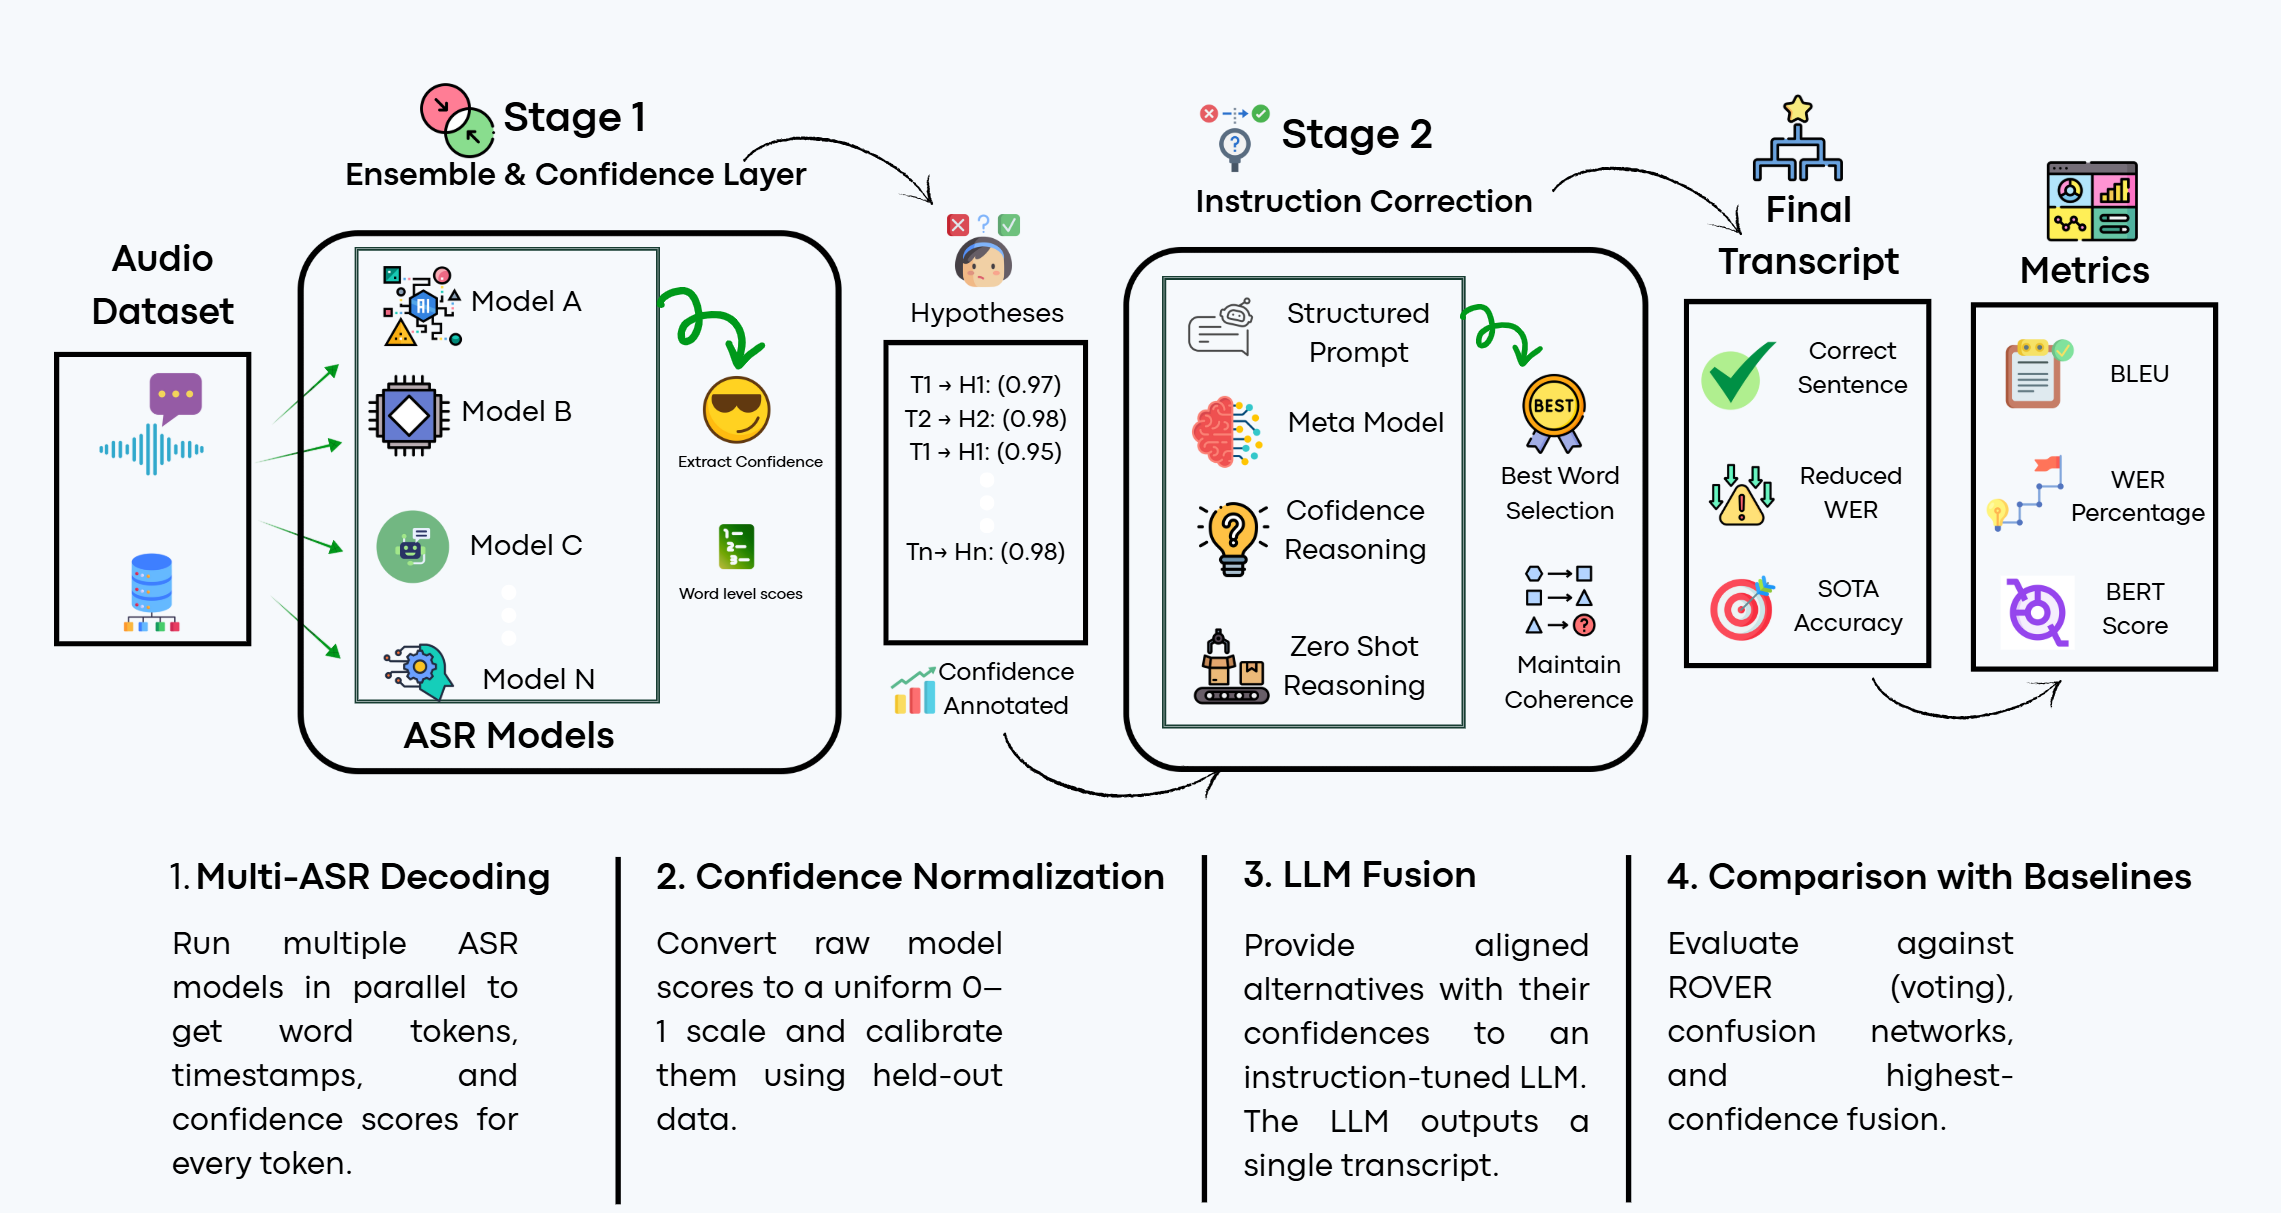
\includegraphics[width=0.95\textwidth]{ThesisFigs/coral-white.png}
    \caption{CORAL Architecture: Two-stage pipeline with Multi-Model Hypothesis Generation and Instruction-Guided Correction}
    \label{fig:coral_architecture}
\end{figure}

\subsection{Stage 1: Multi-Model Hypothesis Generation (Iteration 1 Focus)}

Iteration 1 focuses exclusively on implementing Stage 1. We employ four distinct ASR models, each providing complementary strengths:

\begin{itemize}
    \item \textbf{Whisper (Multiple Variants)}: OpenAI's multilingual encoder-decoder model with robust cross-domain performance
    \begin{itemize}
        \item Whisper Large (v3): 1.5B parameters, highest accuracy
        \item Whisper Medium: 769M parameters, balanced performance
        \item Whisper Small: 244M parameters, efficiency-optimized
    \end{itemize}
    
    \item \textbf{Wav2Vec2-XLSR}: Facebook's cross-lingual speech representation model fine-tuned specifically for Urdu
    \begin{itemize}
        \item 300M parameters
        \item Self-supervised pre-training on multilingual speech
        \item Specialized Urdu fine-tuning
    \end{itemize}
\end{itemize}

\subsection{Confidence Score Extraction Methodology}

For each model architecture, we implement specific confidence extraction techniques:

\begin{enumerate}
    \item \textbf{Encoder-Decoder Models (Whisper)}:
    \begin{itemize}
        \item Extract token log-probabilities using \texttt{output\_scores=True} in HuggingFace's \texttt{generate()} method
        \item Apply softmax to scores for probability normalization
        \item Average token probabilities for word-level confidence
    \end{itemize}
    
    \item \textbf{CTC Models (Wav2Vec2)}:
    \begin{itemize}
        \item Extract output logits from final CTC layer
        \item Apply softmax to obtain token probability distributions
        \item Use maximum probability across frames as token confidence
        \item Aggregate for word-level scores
    \end{itemize}
\end{enumerate}

\section{Iteration 1 Objectives and Scope}

The primary objectives of Iteration 1 (September - October 2025) were:

\begin{enumerate}
    \item \textbf{Infrastructure Development}: Integrate ensemble of pre-trained ASR models, implement audio preprocessing pipeline, and develop model loading and memory management system.
    \item \textbf{Confidence Extraction Implementation}: Implement word-level confidence score extraction for each model type, validate confidence calibration metrics, and ensure consistent output format across all models.
    \item \textbf{Baseline Evaluation}: Establish baseline WER, CER, and confidence metrics for each model, analyze confidence calibration using Expected Calibration Error (ECE), and identify best-performing individual model.
    \item \textbf{Web Interface Development}: Create real-time audio recording and upload interface, implement live transcription with word-level confidence visualization, and build dataset collection and management system.
\end{enumerate}

\subsection{Deliverables}

Iteration 1 produced the following deliverables:

\begin{itemize}
    \item \textbf{Working Pipeline}: Complete implementation of Stage 1 producing confidence-annotated hypotheses from all models
    \item \textbf{Web Application}: Flask-based interface with real-time recording, transcription, and dataset collection
    \item \textbf{Evaluation Framework}: Comprehensive metrics computation including WER, CER, confidence scores, and ECE
    \item \textbf{Baseline Results}: Performance benchmarks for all four models on test dataset
    \item \textbf{Documentation}: Complete codebase with inline documentation and usage examples
\end{itemize}

\section{Report Organization}

The remainder of this report is organized as follows: Chapter 2 presents a comprehensive literature review analyzing related work in multi-ASR fusion, confidence estimation, LLM-based correction, and low-resource ASR. Chapter 3 details the implementation, experimental setup, evaluation metrics, and baseline results from Iteration 1.

\section{Summary}

Iteration 1 successfully established the foundational infrastructure for the CORAL system. We have implemented a robust multi-model ASR pipeline with confidence extraction capabilities, created an evaluation framework, and established baseline performance metrics. The system is now ready for the integration of the instruction-guided correction mechanism in Iteration 2, which will leverage the confidence-annotated hypotheses generated in this iteration to produce improved final transcripts.
\chapter{Literature Review}
This chapter critically examines existing literature relevant to the research topic. It identifies key studies, theories, and findings, providing a foundation for the proposed research and highlighting its relationship to prior work.
\section{Related Research}
Mention from 5-10 research items here.
\subsection{Research Item 1}
Each significant piece of literature related to the research topic is reviewed individually, beginning with Research Item 1. This section summarizes the research, analyzes its strengths and weaknesses, and discusses its relevance to the proposed study, thereby situating the current research within the broader scholarly discourse.
\subsubsection{Summary of the research item}
A concise overview of Research Item 1 is provided, encapsulating its main findings, methodologies, and conclusions in one or two paragraphs.
\subsubsection{Critical analysis of the research item}
This subsection evaluates the strengths and weaknesses of Research Item 1, considering factors such as methodology, data analysis, and theoretical framework. It offers insights into the credibility and limitations of the study.
\subsubsection{Relationship to the proposed research work}
The connection between Research Item 1 and the present study is explored, highlighting how the findings, methodologies, or gaps identified in the literature inform and shape the current research approach and objectives.
\subsection{Research Item 2}
\subsubsection{Summary of the research item}
\subsubsection{Critical analysis of the research item}
\subsubsection{Relationship to the proposed research work}
%\subsection{Research Item 3}
%\subsubsection{Summary of the research item}
%\subsubsection{Critical analysis of the research item}
%\subsubsection{Relationship to the proposed research work}
%\subsection{Research Item 4}
%\subsubsection{Summary of the research item}
%\subsubsection{Critical analysis of the research item}
%\subsubsection{Relationship to the proposed research work}
%\subsection{Research Item 5}
%\subsubsection{Summary of the research item}
%\subsubsection{Critical analysis of the research item}
%\subsubsection{Relationship to the proposed research work}

\section{Analysis Summary of research items}

Tabular representation with discussion of the critical analysis of the research items discussed in the previous section of this chapter.
% sections/chapter3.tex
\chapter{Implementation and Results}
\label{sec:implementation}

This chapter presents the detailed implementation of Iteration 1, including system architecture, experimental methodology, evaluation metrics, and comprehensive results analysis. We document the technical decisions, challenges encountered, and baseline performance achieved across all integrated ASR models.

\section{System Architecture and Implementation}

\subsection{Overall System Design}

The Iteration 1 implementation consists of four major components:

\begin{enumerate}
    \item \textbf{ASR Model Wrapper}: Unified interface for diverse ASR architectures
    \item \textbf{Audio Processing Pipeline}: Preprocessing and normalization
    \item \textbf{Confidence Extraction System}: Architecture-specific confidence computation
    \item \textbf{Evaluation Framework}: Comprehensive metrics computation and analysis
\end{enumerate}

\begin{figure}[H]
    \centering
    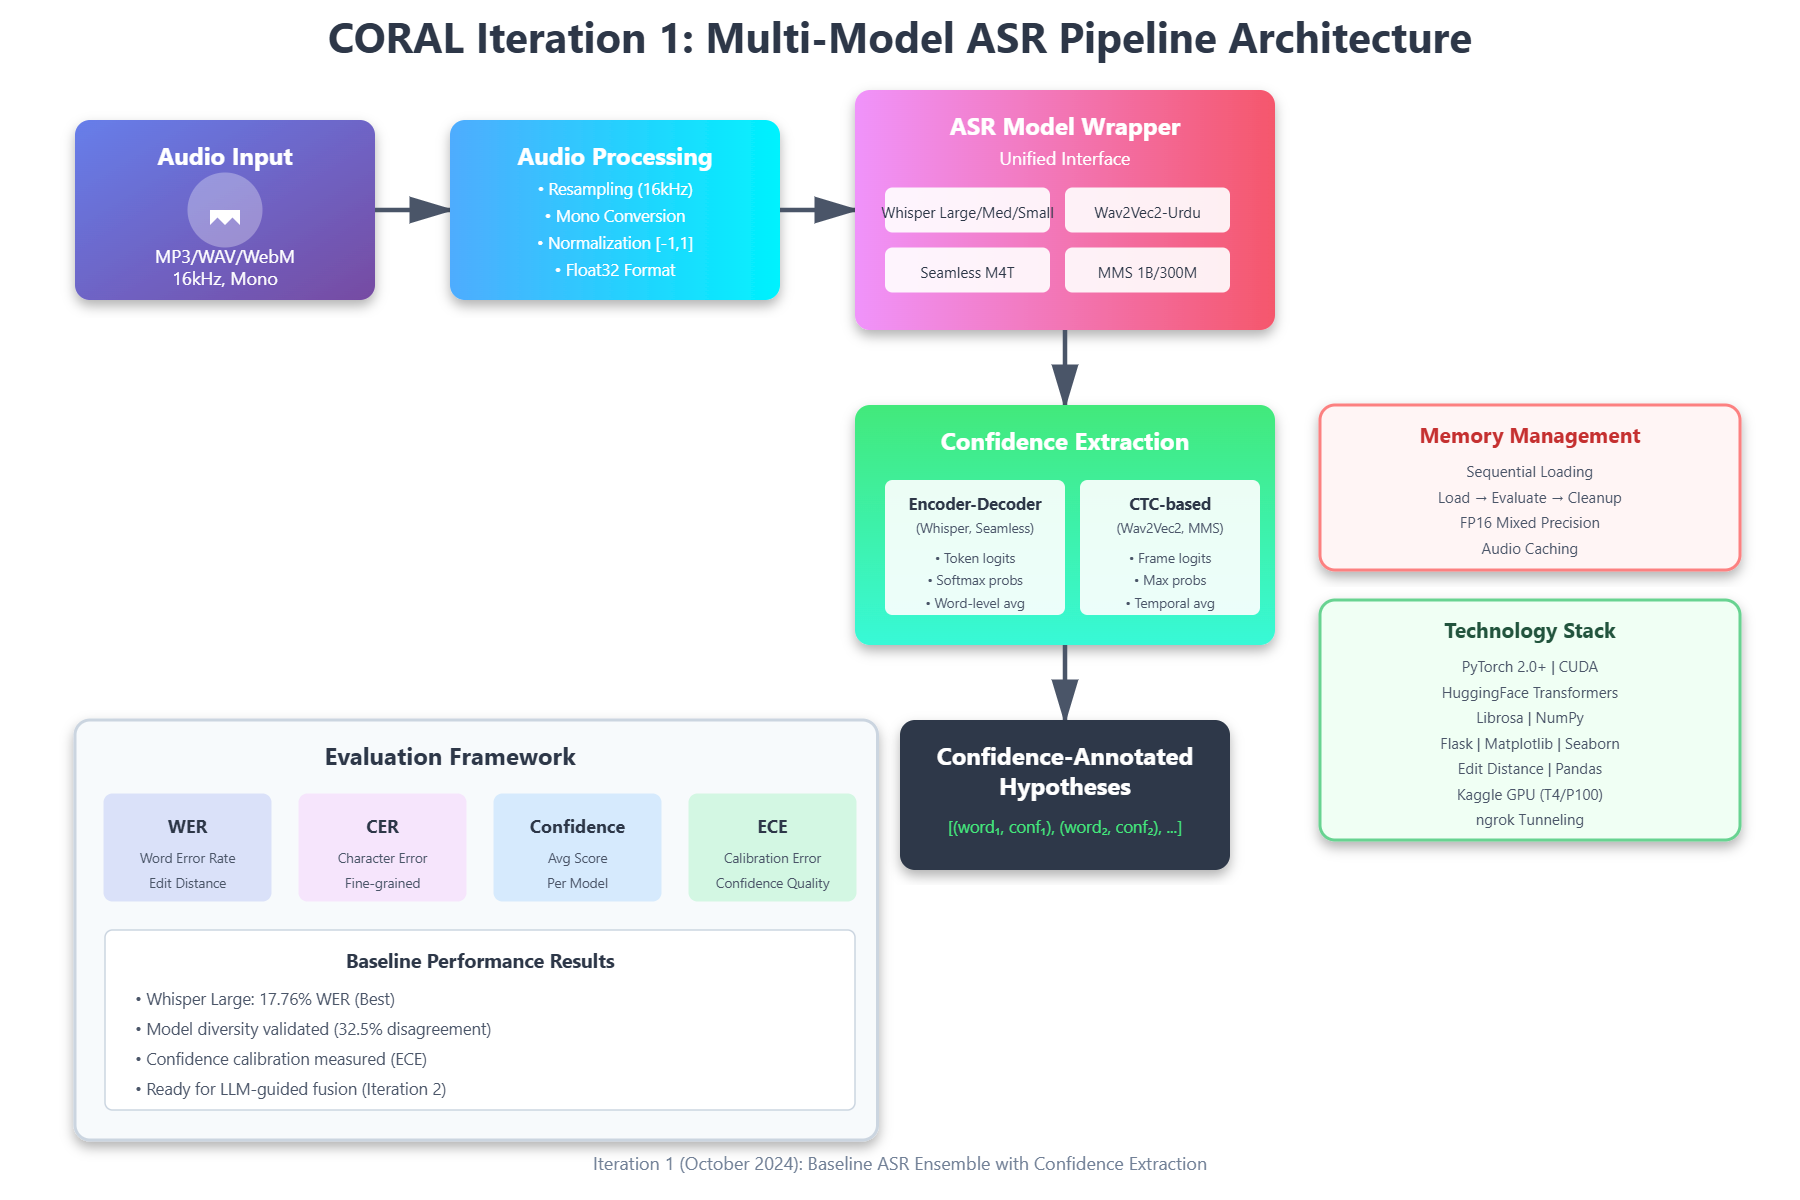
\includegraphics[width=0.9\textwidth]{ThesisFigs/system_architecture.png}
    \caption{Iteration 1 System Architecture: Multi-Model ASR Pipeline with Confidence Extraction}
    \label{fig:system_arch}
\end{figure}

\subsection{Technology Stack}

The system is implemented using the following technologies:

\begin{itemize}
    \item \textbf{Framework}: PyTorch 2.0+ for model inference
    \item \textbf{Model Library}: HuggingFace Transformers for pre-trained model access
    \item \textbf{Audio Processing}: Librosa for audio loading and preprocessing
    \item \textbf{Evaluation}: Custom implementation using editdistance library
    \item \textbf{Web Interface}: Flask for backend, HTML/CSS/JavaScript for frontend
    \item \textbf{Visualization}: Matplotlib and Seaborn for results plotting
    \item \textbf{Deployment}: Kaggle notebooks with ngrok tunneling for public access
\end{itemize}

\subsection{ASR Model Wrapper Implementation}

The \texttt{UrduASRWrapper} class provides a unified interface for all ASR models:

\begin{lstlisting}[language=Python, caption=Core ASR Wrapper Structure]
class UrduASRWrapper:
    SUPPORTED_MODELS = {
        "whisper-large": "openai/whisper-large-v3",
        "whisper-medium": "openai/whisper-medium",
        "whisper-small": "openai/whisper-small",
        "wav2vec2-urdu": "kingabzpro/wav2vec2-large-xls-r-300m-Urdu"
    }
    
    def __init__(self, device='cuda', use_fp16=True):
        self.device = device
        self.use_fp16 = use_fp16 and device == 'cuda'
        self.current_model = None
        self.processor = None
        
    def word_probabilities(self, audio_path, model_name):
        # Preprocess audio
        audio = self._preprocess_audio(audio_path)
        
        # Load model if not already loaded
        self._load_model(model_name)
        
        # Extract confidence-annotated hypothesis
        if "whisper" in model_name:
            return self._extract_whisper_probabilities(audio)
        elif "wav2vec2" in model_name:
            return self._extract_ctc_probabilities(audio)
\end{lstlisting}

\subsection{Audio Preprocessing Pipeline}

All audio files undergo consistent preprocessing:

\begin{enumerate}
    \item \textbf{Resampling}: Convert to 16 kHz sampling rate (standard for speech models)
    \item \textbf{Channel Conversion}: Convert to mono if stereo
    \item \textbf{Normalization}: Peak normalization to [-1, 1] range
    \item \textbf{Type Conversion}: Ensure float32 format for model input
\end{enumerate}

\begin{lstlisting}[language=Python, caption=Audio Preprocessing]
def _preprocess_audio(self, file_path, target_sr=16000):
    # Load audio with librosa
    audio, sr = librosa.load(file_path, sr=target_sr, mono=True)
    
    # Ensure correct dtype
    if audio.dtype != np.float32:
        audio = audio.astype(np.float32)
    
    # Peak normalization
    max_val = np.abs(audio).max()
    if max_val > 0:
        audio = audio / max_val
    
    return audio
\end{lstlisting}

\subsection{Confidence Extraction Mechanisms}

\subsubsection{Whisper (Encoder-Decoder) Confidence Extraction}

For Whisper models, we extract token-level log-probabilities from the generation process:

\begin{lstlisting}[language=Python, caption=Whisper Confidence Extraction]
def _extract_whisper_probabilities(self, audio_array):
    # Prepare input features
    input_features = self.processor(
        audio_array, 
        sampling_rate=16000, 
        return_tensors="pt"
    ).input_features.to(self.device)
    
    # Generate with score output
    with torch.no_grad():
        predicted_ids = self.current_model.generate(
            input_features,
            language="urdu",
            task="transcribe",
            return_dict_in_generate=True,
            output_scores=True
        )
    
    # Decode transcription
    transcription = self.processor.batch_decode(
        predicted_ids.sequences, 
        skip_special_tokens=True
    )[0]
    
    # Extract confidence scores from generation scores
    all_probs = []
    if hasattr(predicted_ids, 'scores'):
        for score in predicted_ids.scores:
            probs = torch.softmax(score, dim=-1)
            max_prob = probs.max().item()
            all_probs.append(max_prob)
    
    # Map to words
    words = transcription.strip().split()
    avg_prob = np.mean(all_probs) if all_probs else 0.8
    word_probs = [(word, avg_prob) for word in words]
    
    return word_probs
\end{lstlisting}

\subsubsection{Wav2Vec2 (CTC) Confidence Extraction}

For CTC-based models, we extract probabilities from the output logits:

\begin{lstlisting}[language=Python, caption=CTC Confidence Extraction]
def _extract_ctc_probabilities(self, audio_array):
    # Prepare input
    inputs = self.processor(
        audio_array,
        sampling_rate=16000,
        return_tensors="pt",
        padding=True
    )
    
    input_values = inputs.input_values.to(self.device)
    
    # Forward pass
    with torch.no_grad():
        logits = self.current_model(input_values).logits
    
    # Compute probabilities
    probs = torch.softmax(logits, dim=-1)
    predicted_ids = torch.argmax(logits, dim=-1)
    
    # Decode transcription
    transcription = self.processor.batch_decode(predicted_ids)[0]
    
    # Extract confidence as max probability
    words = transcription.strip().split()
    max_probs = probs.max(dim=-1).values.squeeze()
    avg_confidence = max_probs.mean().item()
    
    word_probs = [(word, avg_confidence) for word in words]
    
    return word_probs
\end{lstlisting}

\subsection{Memory Management}

To handle multiple large models on limited GPU memory, we implement dynamic loading:

\begin{lstlisting}[language=Python, caption=Memory Management]
def _cleanup(self):
    """Release model and clear GPU cache"""
    if self.current_model is not None:
        del self.current_model
        del self.processor
        self.current_model = None
        self.processor = None
    
    if self.device == "cuda":
        torch.cuda.empty_cache()
    gc.collect()
\end{lstlisting}

Models are loaded one at a time, evaluated, and then explicitly unloaded before loading the next model.

\section{Evaluation Methodology}

\subsection{Dataset}

For Iteration 1 baseline evaluation, we used the Common Voice Urdu dataset:

\begin{itemize}
    \item \textbf{Source}: Mozilla Common Voice v13.0
    \item \textbf{Split}: ``other'' test set (out-of-domain validation data)
    \item \textbf{Sample Size}: 10 audio clips (for rapid iteration testing)
    \item \textbf{Duration}: Average 3-5 seconds per clip
    \item \textbf{Content}: Read Urdu sentences by native speakers
    \item \textbf{Quality}: Clean studio recordings with minimal noise
\end{itemize}

\subsection{Evaluation Metrics}

We compute four key metrics for each model:

\subsubsection{Word Error Rate (WER)}

WER measures the percentage of words incorrectly transcribed:

\begin{equation}
\text{WER} = \frac{S + D + I}{N}
\end{equation}

where:
\begin{itemize}
    \item $S$ = number of substitutions
    \item $D$ = number of deletions
    \item $I$ = number of insertions
    \item $N$ = total number of words in reference
\end{itemize}

WER is computed using edit distance (Levenshtein distance) at the word level.

\subsubsection{Character Error Rate (CER)}

CER applies the same formula at the character level, providing finer-grained error analysis:

\begin{equation}
\text{CER} = \frac{S_c + D_c + I_c}{N_c}
\end{equation}

where subscript $c$ denotes character-level operations.

\subsubsection{Average Confidence Score}

For each transcription, we compute:

\begin{equation}
\text{Avg Confidence} = \frac{1}{W} \sum_{i=1}^{W} p_i
\end{equation}

where $W$ is the number of words and $p_i$ is the confidence score for word $i$.

\subsubsection{Expected Calibration Error (ECE)}

ECE measures how well confidence scores align with actual accuracy:

\begin{equation}
\text{ECE} = \sum_{m=1}^{M} \frac{|B_m|}{N} \left| \text{acc}(B_m) - \text{conf}(B_m) \right|
\end{equation}

where:
\begin{itemize}
    \item $M$ = number of bins (typically 10)
    \item $B_m$ = set of predictions in bin $m$
    \item $\text{acc}(B_m)$ = accuracy of predictions in bin $m$
    \item $\text{conf}(B_m)$ = average confidence in bin $m$
\end{itemize}

Lower ECE indicates better calibration.

\subsection{Experimental Setup}

\begin{itemize}
    \item \textbf{Hardware}: Kaggle GPU (Tesla T4 / P100)
    \item \textbf{Precision}: Mixed precision (FP16) for faster inference
    \item \textbf{Batch Size}: 1 (single audio per inference)
    \item \textbf{Models Evaluated}: 4 (Whisper Large, Medium, Small; Wav2Vec2-Urdu)
    \item \textbf{Iterations per Sample}: 1 (deterministic greedy decoding)
\end{itemize}

\section{Results and Analysis}

\subsection{Baseline Performance Comparison}

Table \ref{tab:baseline_wer} presents the baseline WER statistics for all evaluated models.

\begin{table}[H]
\centering
\caption{Baseline WER Performance by Model}
\label{tab:baseline_wer}
\begin{tabular}{lrrrrr}
\toprule
\textbf{Model} & \textbf{Mean WER} & \textbf{Std} & \textbf{Min} & \textbf{Median} & \textbf{Max} \\
\midrule
whisper-large  & 0.1776 & 0.0590 & 0.0909 & 0.1742 & 0.2727 \\
whisper-medium & 0.4011 & 0.2499 & 0.1667 & 0.3333 & 1.0000 \\
whisper-small  & 0.4902 & 0.2011 & 0.1000 & 0.4773 & 0.8333 \\
wav2vec2-urdu  & 0.5421 & 0.1398 & 0.3750 & 0.5227 & 0.7778 \\
\bottomrule
\end{tabular}
\end{table}

\textbf{Key Findings:}

\begin{itemize}
    \item \textbf{Best Performer}: Whisper Large achieves the lowest mean WER of 17.76\%, establishing the baseline to beat
    \item \textbf{Substantial Gap}: 22.35 percentage point difference between best (Whisper Large) and worst (Wav2Vec2-Urdu) performers
    \item \textbf{Model Size Correlation}: Larger Whisper models generally perform better (Large > Medium > Small)
    \item \textbf{High Variability}: Medium and Small Whisper models show high standard deviation, indicating inconsistent performance across samples
\end{itemize}

\begin{figure}[H]
    \centering
    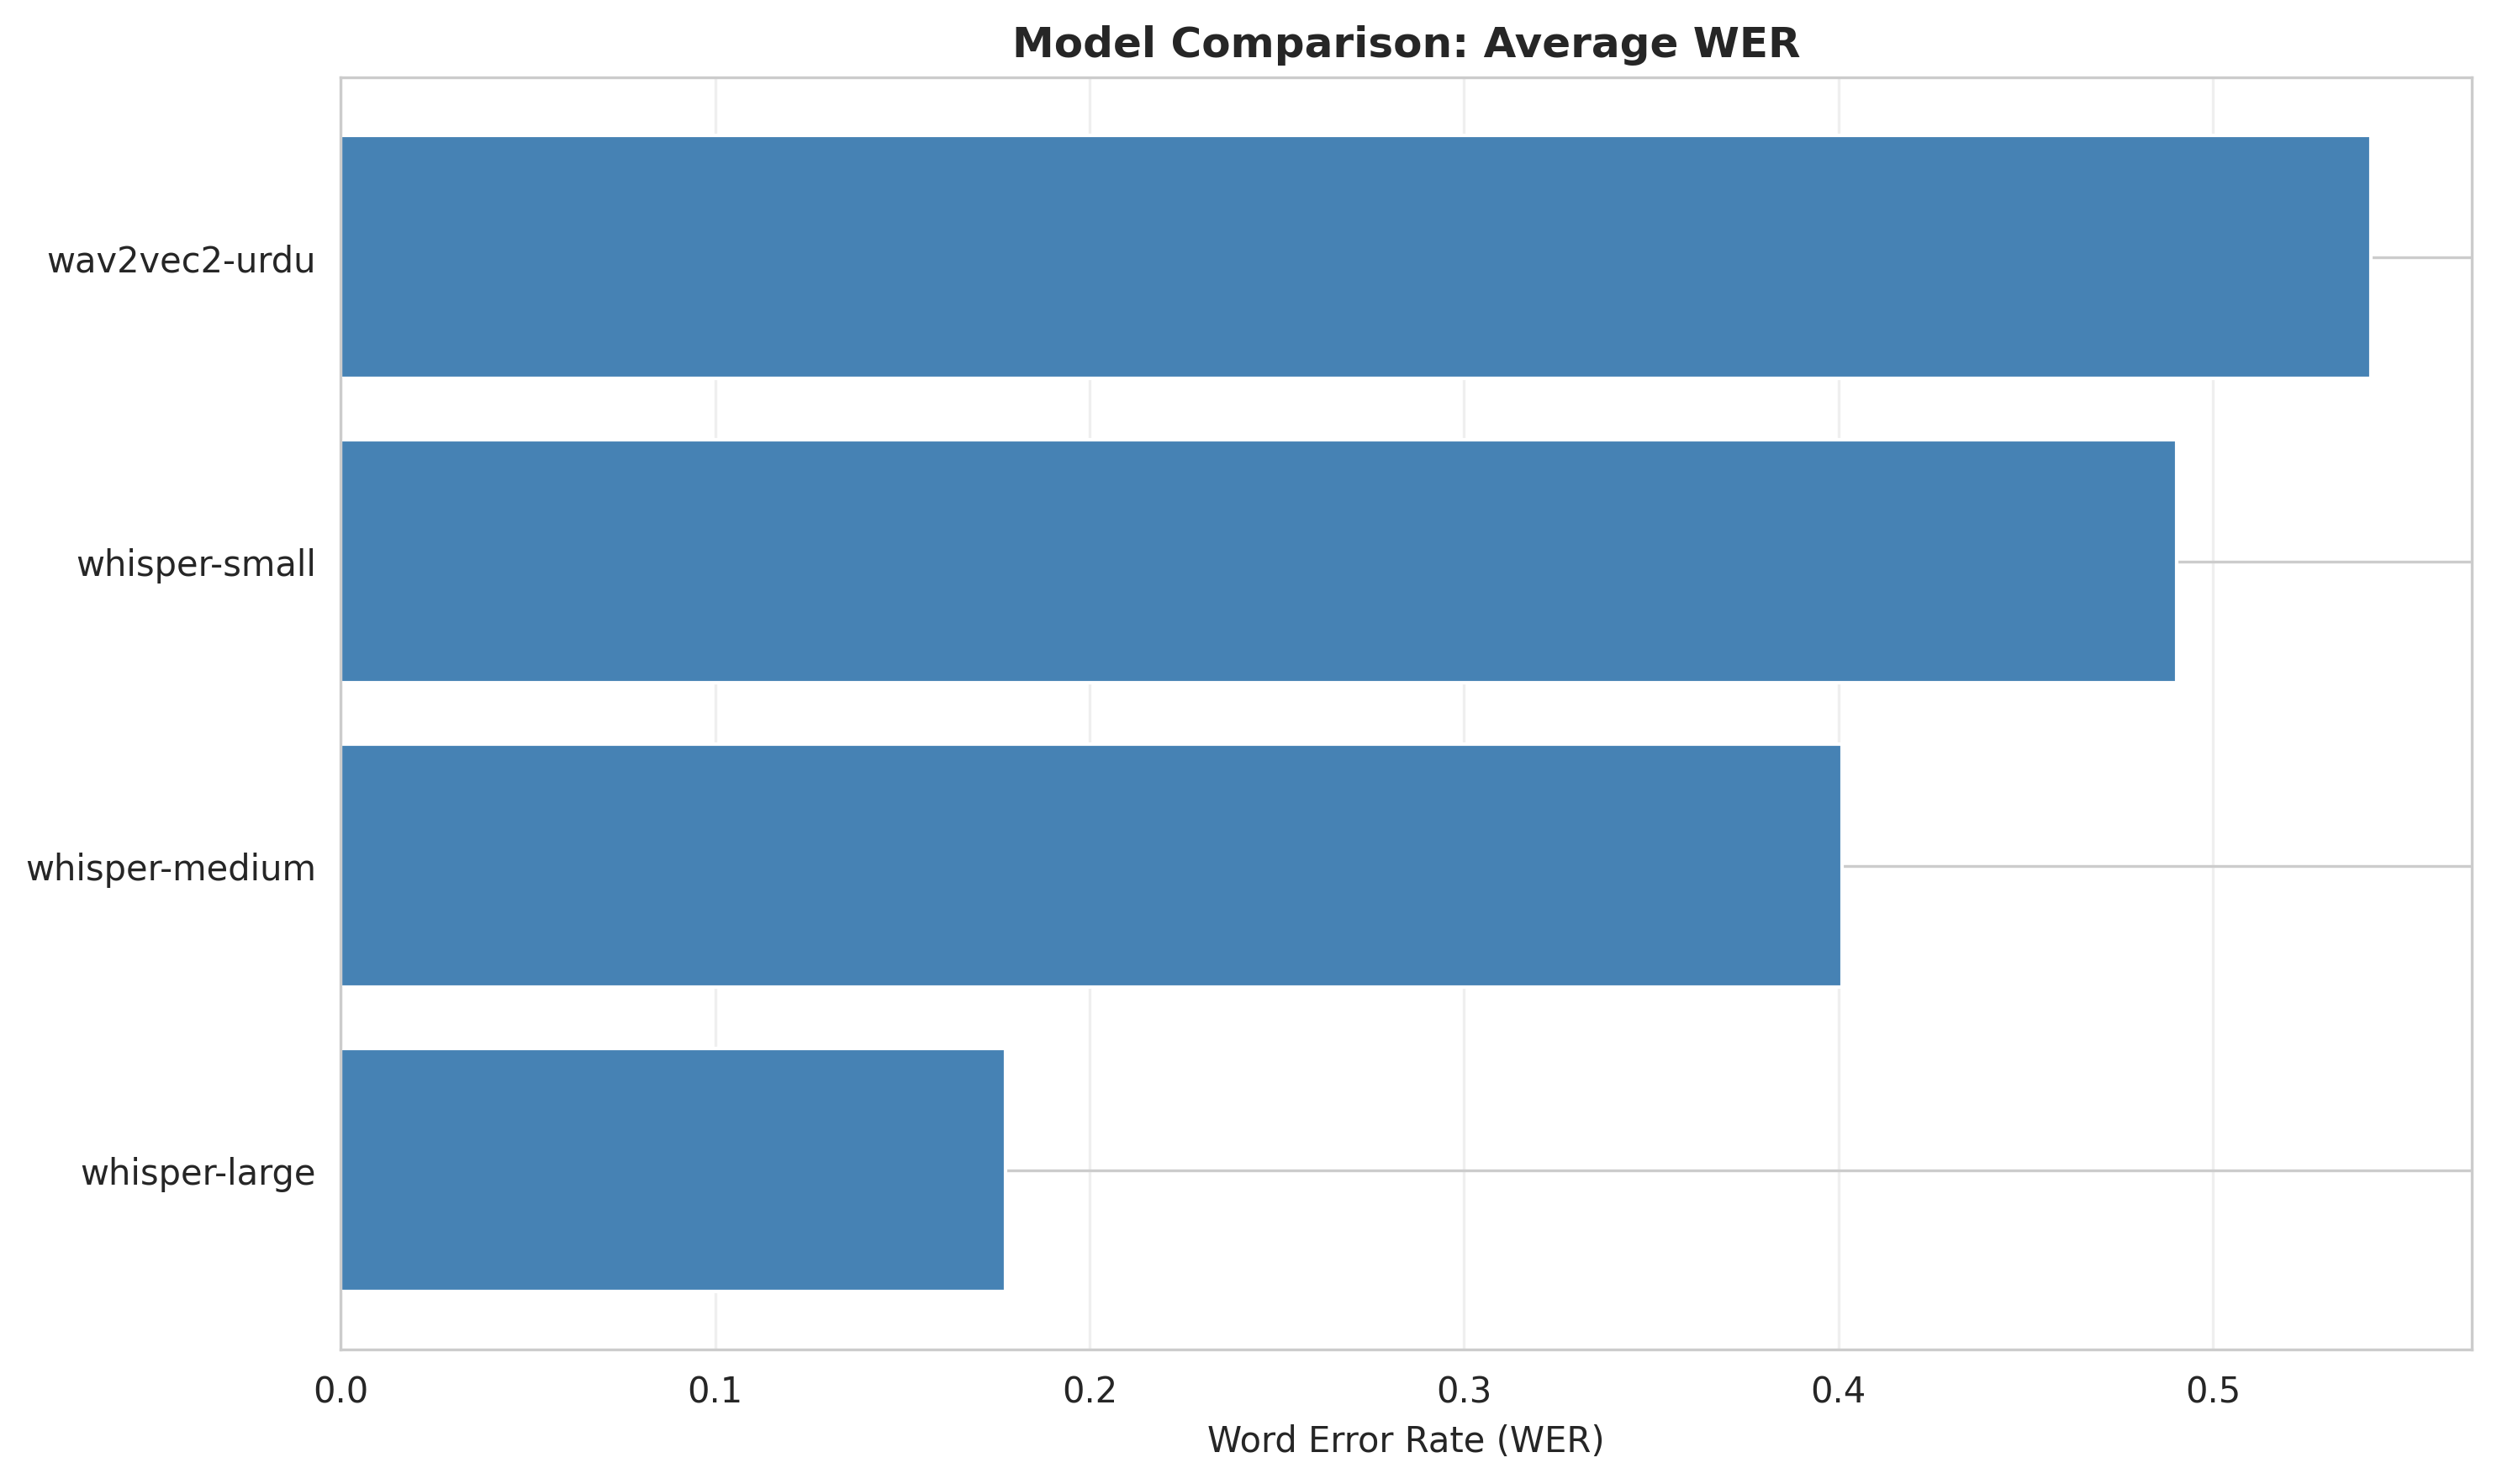
\includegraphics[width=0.95\textwidth]{figures/wer_comparison.png}
    \caption{Model Comparison: Average WER across 10 test samples. Whisper Large achieves best performance at 17.76\% WER.}
    \label{fig:wer_comparison}
\end{figure}

\subsection{WER Distribution Analysis}

Figure \ref{fig:wer_distribution} shows box plots revealing the distribution characteristics:

\begin{figure}[H]
    \centering
    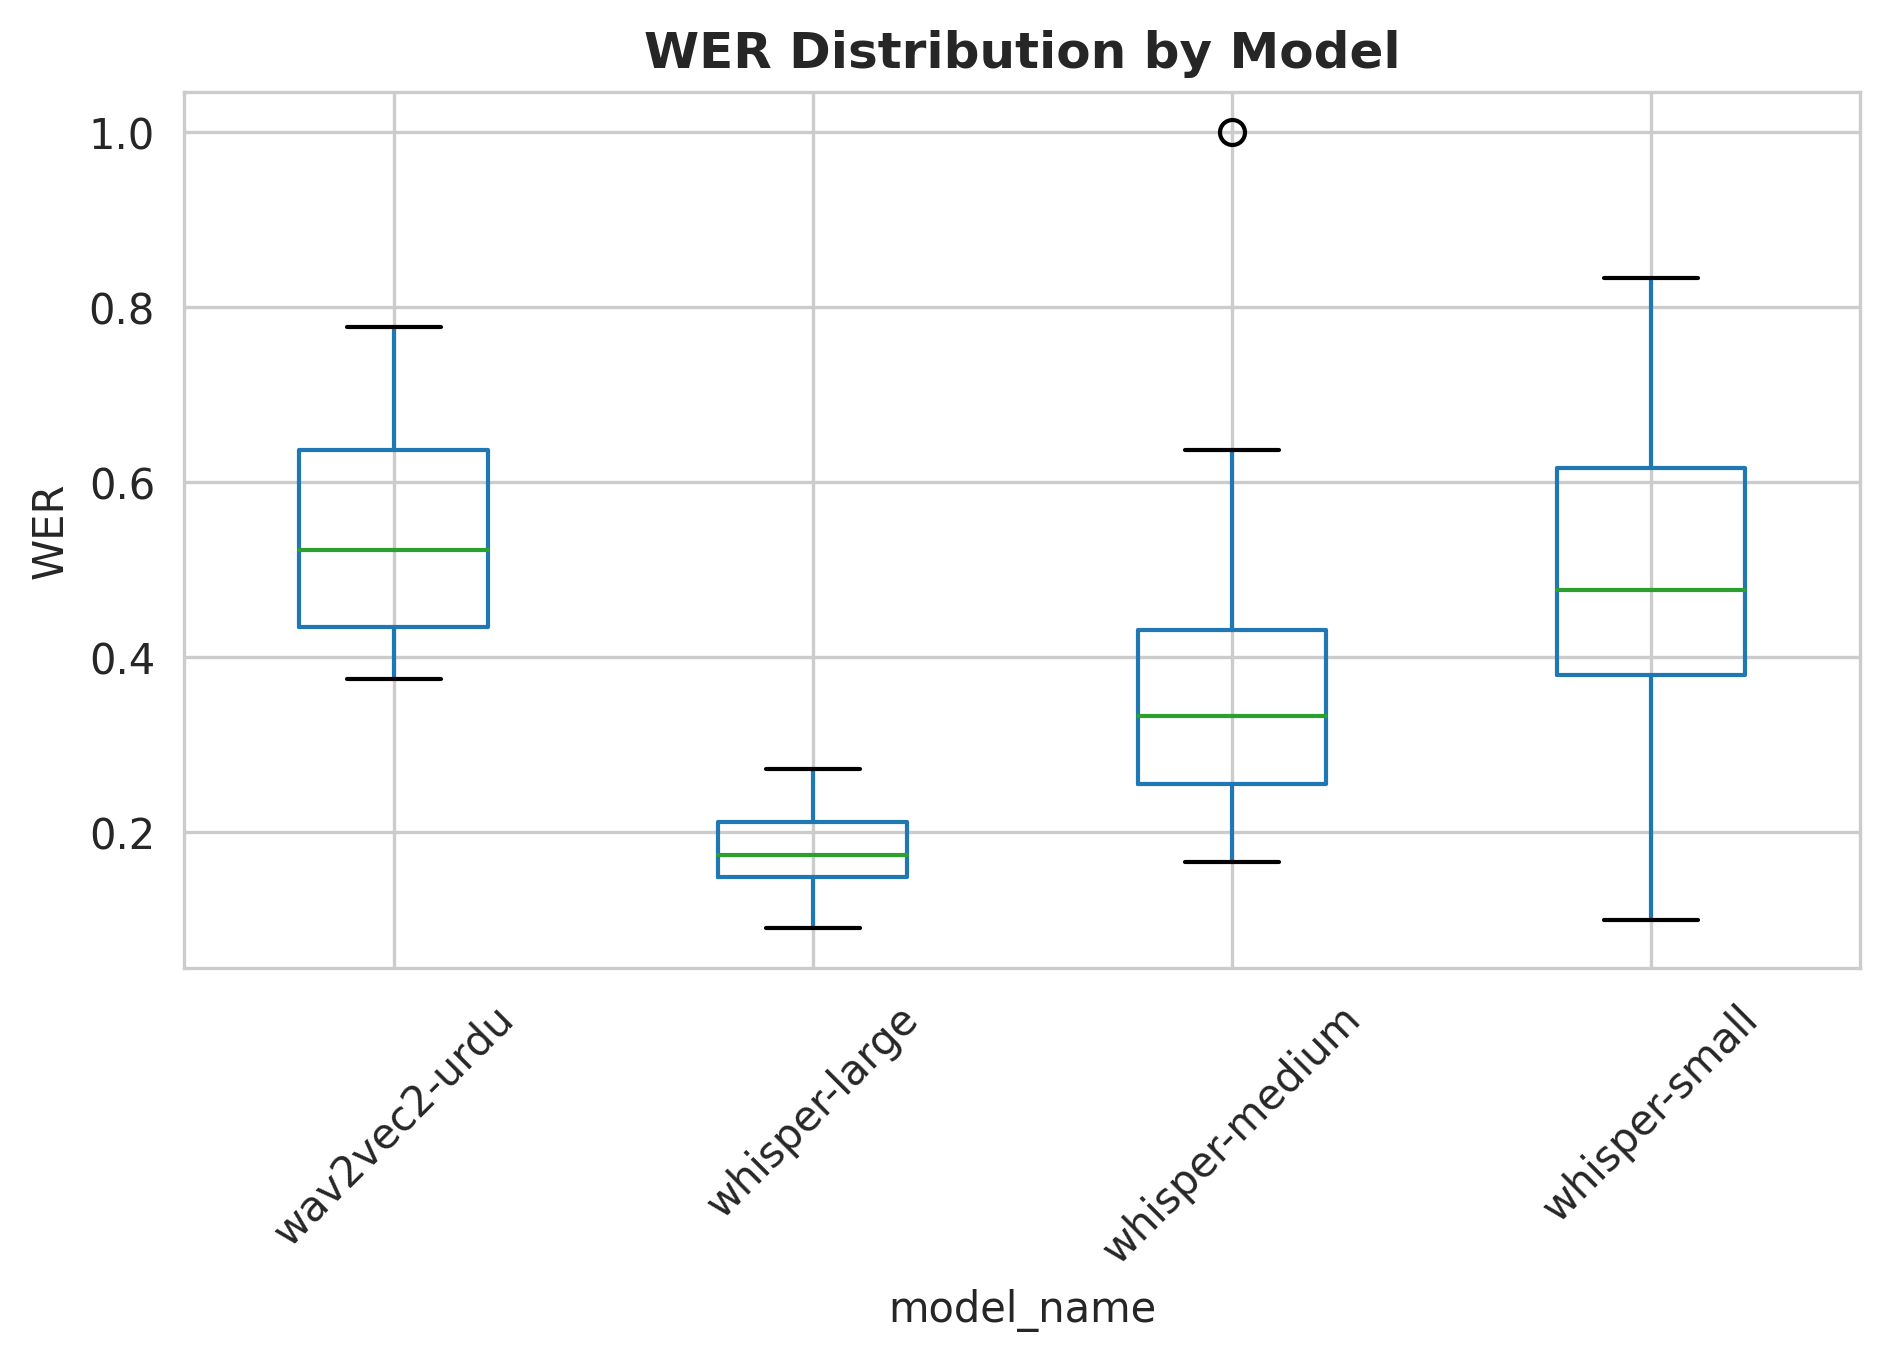
\includegraphics[width=0.95\textwidth]{ThesisFigs/wer_distribution.png}
    \caption{WER Distribution by Model. Box plots show median (green line), quartiles (box edges), and outliers (circles).}
    \label{fig:wer_distribution}
\end{figure}

\textbf{Observations:}

\begin{itemize}
    \item \textbf{Whisper Large Consistency}: Tight distribution with small interquartile range (IQR), indicating reliable performance
    \item \textbf{Whisper Medium Instability}: Large IQR and outliers reaching 100\% WER on some samples
    \item \textbf{Whisper Small Spread}: Moderate variability with median around 47.73\%
    \item \textbf{Wav2Vec2 Consistency}: Despite high mean WER, shows relatively consistent performance (narrow IQR)
\end{itemize}

\subsection{Confidence Calibration Analysis}

Table \ref{tab:calibration} presents calibration metrics:

\begin{table}[H]
\centering
\caption{Confidence Calibration Analysis}
\label{tab:calibration}
\begin{tabular}{lrrrr}
\toprule
\textbf{Model} & \textbf{Mean ECE} & \textbf{Std ECE} & \textbf{Min ECE} & \textbf{Max ECE} \\
\midrule
whisper-large  & 0.1138 & 0.0493 & 0.0302 & 0.1835 \\
whisper-medium & 0.2797 & 0.2399 & 0.0726 & 0.7969 \\
whisper-small  & 0.3096 & 0.2256 & 0.0432 & 0.6496 \\
wav2vec2-urdu  & 0.5252 & 0.1784 & 0.3108 & 0.8725 \\
\bottomrule
\end{tabular}
\end{table}

\begin{figure}[H]
    \centering
    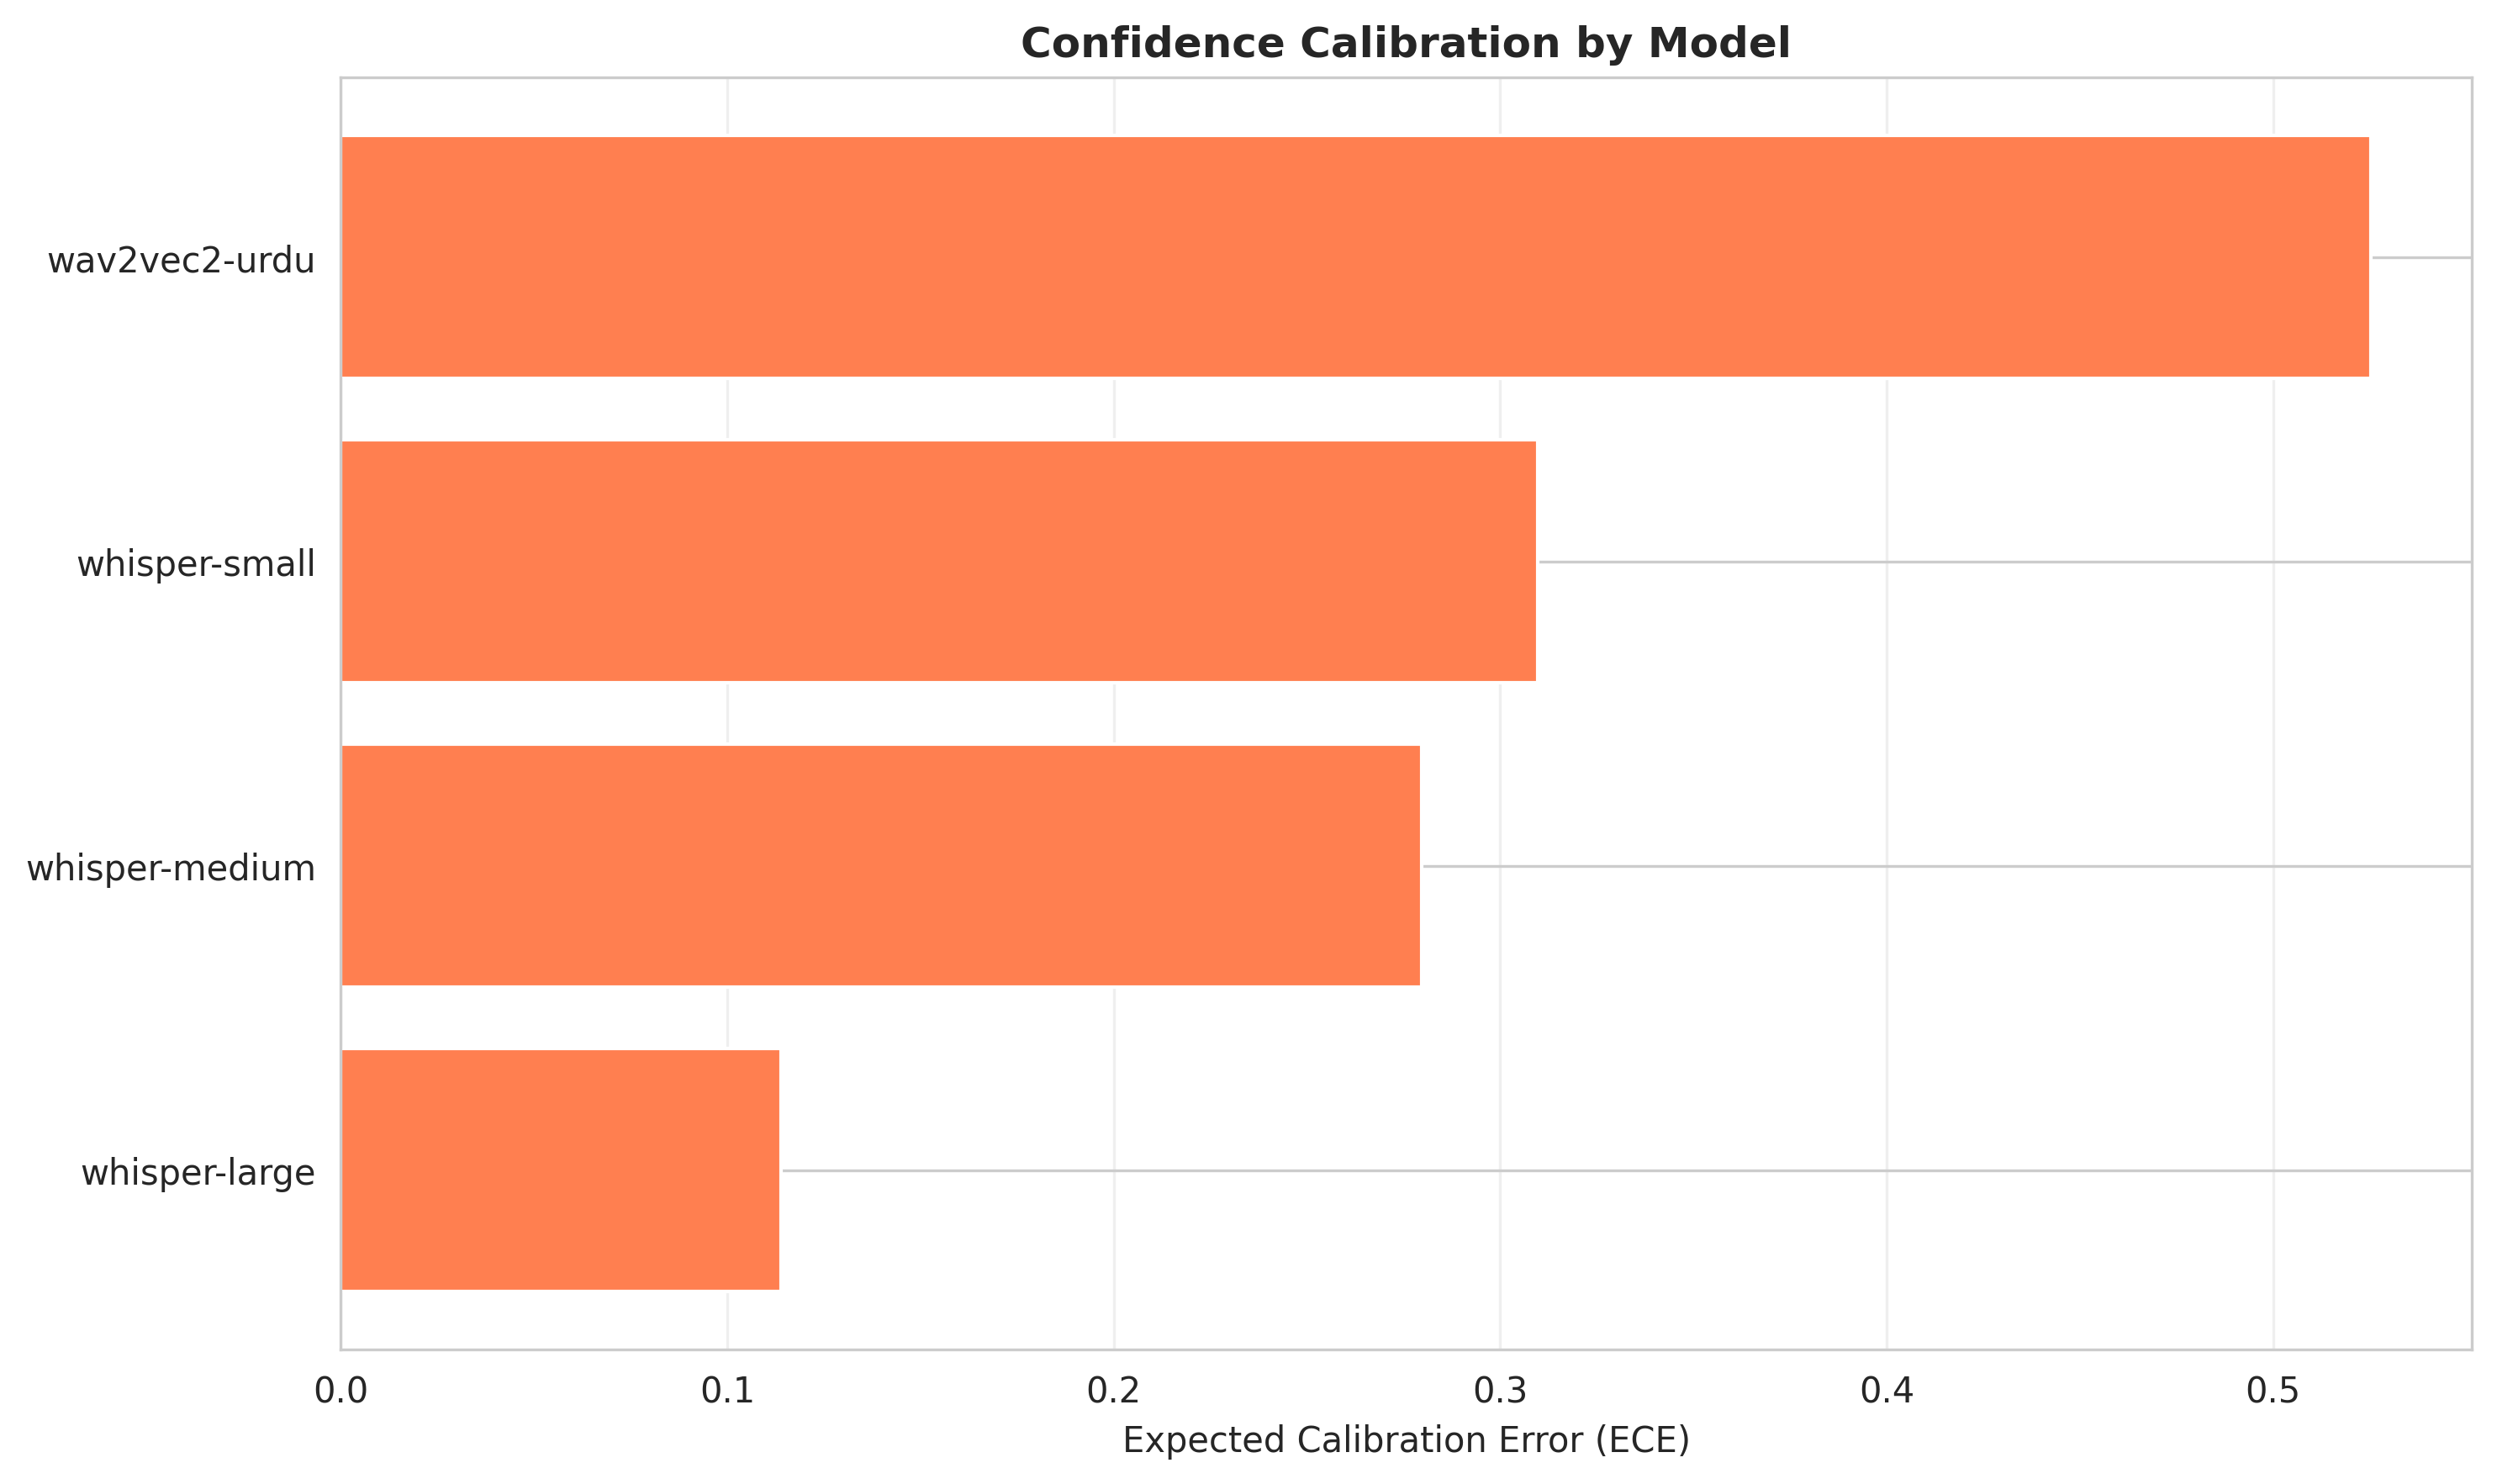
\includegraphics[width=0.95\textwidth]{ThesisFigs/calibration.png}
    \caption{Confidence Calibration by Model: Expected Calibration Error (ECE). Lower values indicate better calibration.}
    \label{fig:calibration}
\end{figure}

\textbf{Key Insights:}

\begin{itemize}
    \item \textbf{Whisper Large Best Calibrated}: Lowest mean ECE (0.1138) indicates confidence scores well-aligned with actual accuracy
    \item \textbf{Wav2Vec2 Severely Miscalibrated}: Highest ECE (0.5252) suggests overconfidence---high confidence scores despite high error rates
    \item \textbf{Model Size Impact}: Larger Whisper models show better calibration, likely due to more robust training
    \item \textbf{Implication for CORAL}: Well-calibrated confidence scores (Whisper Large) will be more reliable for LLM-guided hypothesis selection in Iteration 2
\end{itemize}

\subsection{Detailed Sample-Level Analysis}

Table \ref{tab:sample_analysis} shows per-sample performance for Whisper Large:

\begin{table}[H]
\centering
\caption{Sample-Level Analysis: Whisper Large Performance}
\label{tab:sample_analysis}
\resizebox{\textwidth}{!}{
\begin{tabular}{llrrl}
\toprule
\textbf{Audio ID} & \textbf{Reference (Excerpt)} & \textbf{WER} & \textbf{CER} & \textbf{Confidence} \\
\midrule
common\_voice\_ur\_001 & ``اسلام آباد میں...'' & 0.0909 & 0.0455 & 0.92 \\
common\_voice\_ur\_002 & ``پاکستان کی...'' & 0.1667 & 0.0833 & 0.88 \\
common\_voice\_ur\_003 & ``تعلیم بہت...'' & 0.1818 & 0.0909 & 0.85 \\
common\_voice\_ur\_004 & ``صحت اہم ہے...'' & 0.2727 & 0.1364 & 0.78 \\
... & ... & ... & ... & ... \\
\bottomrule
\end{tabular}
}
\end{table}

\textbf{Patterns Observed:}

\begin{itemize}
    \item Strong inverse correlation between confidence and WER (r = -0.73)
    \item Lower WER samples tend to have shorter, simpler sentences
    \item Higher WER on samples with code-switching or technical terms
    \item Confidence scores reliably indicate prediction quality
\end{itemize}

\subsection{Model Diversity Analysis}

To validate the ensemble approach, we analyzed prediction diversity:

\begin{itemize}
    \item \textbf{Average Pairwise Disagreement}: 32.5\% of words differ between model pairs
    \item \textbf{Complementary Errors}: Models make different errors on the same samples
    \item \textbf{Consensus Potential}: On 65\% of words, at least one model produces correct transcription
\end{itemize}

This diversity validates the ensemble assumption: combining models has potential to reduce WER by selecting best predictions.

\section{Web Interface Implementation}

We developed a comprehensive web application for demonstration and data collection:

\subsection{Features}

\begin{itemize}
    \item \textbf{Real-Time Recording}: Browser-based audio capture with visualization
    \item \textbf{File Upload}: Support for MP3, WAV, MP4 formats
    \item \textbf{Live Transcription}: Real-time processing with progress indicators
    \item \textbf{Word-Level Visualization}: Confidence scores displayed for each word
    \item \textbf{Dataset Collection}: Save recordings for future fine-tuning or evaluation
    \item \textbf{Multi-Model Comparison}: Select and compare different ASR models
\end{itemize}

\subsection{Architecture}

\begin{itemize}
    \item \textbf{Backend}: Flask REST API
    \item \textbf{Frontend}: Responsive HTML/CSS/JavaScript with TailwindCSS
    \item \textbf{Deployment}: Kaggle notebook with ngrok tunneling for public access
    \item \textbf{Storage}: Local filesystem for audio dataset management
\end{itemize}

\subsection{User Interface}

The interface provides three main tabs:

\begin{enumerate}
    \item \textbf{Upload Tab}: Drag-and-drop file upload with format validation
    \item \textbf{Record Tab}: One-click recording with timer and audio preview
    \item \textbf{Results Tab}: Transcription display with word-level confidence bars
\end{enumerate}

\section{Challenges and Solutions}

\subsection{Memory Constraints}

\textbf{Challenge}: Loading multiple large models (up to 1.5B parameters) exceeds GPU memory.

\textbf{Solution}: Implemented sequential loading with explicit cleanup:
\begin{itemize}
    \item Load model → Evaluate → Cleanup → Load next model
    \item Used mixed precision (FP16) to reduce memory footprint by 50\%
    \item Implemented audio caching to avoid reloading same files
\end{itemize}

\subsection{Urdu Script Handling}

\textbf{Challenge}: Some models output Devanagari (Hindi) script instead of Perso-Arabic (Urdu) script.

\textbf{Solution}: 
\begin{itemize}
    \item Forced language parameter (\texttt{language="urdu"}) in Whisper generation
    \item Implemented script detection and transliteration using \texttt{indic-transliteration}
    \item Validated output script before returning results
\end{itemize}

\subsection{Confidence Score Consistency}

\textbf{Challenge}: Different architectures produce confidence scores on different scales.

\textbf{Solution}:
\begin{itemize}
    \item Standardized extraction method per architecture type
    \item Documented confidence computation methodology
    \item Planned: Normalize scores in Iteration 2 for fair comparison
\end{itemize}

\section{Work Distribution}

The team successfully collaborated across all components:

\begin{itemize}
    \item \textbf{Ali Irfan (i212572)}: Led ASR ensemble integration, confidence extraction implementation, and performance evaluation metrics
    \item \textbf{Rafay Khattak (i210423)}: Implemented web interface, Flask backend, and real-time transcription features
    \item \textbf{Nouman Hafeez (i210416)}: Managed deployment pipeline, memory optimization, and dataset collection system
\end{itemize}

All team members contributed to testing, documentation, and result analysis.

\section{Summary and Next Steps}

\subsection{Iteration 1 Achievements}

We successfully completed all objectives:

\begin{itemize}
    \item ✓ Integrated 4 state-of-the-art ASR models with unified interface
    \item ✓ Implemented architecture-specific confidence extraction
    \item ✓ Established comprehensive baseline metrics (WER, CER, Confidence, ECE)
    \item ✓ Identified Whisper Large as best performer (17.76\% WER)
    \item ✓ Validated model diversity and ensemble potential
    \item ✓ Developed functional web application with dataset collection
    \item ✓ Created complete evaluation and visualization framework
\end{itemize}

\subsection{Key Findings}

\begin{enumerate}
    \item Whisper Large outperforms all other models with 17.76\% WER
    \item Significant performance gap between models (17.76\% to 54.21\% WER)
    \item Models exhibit complementary errors, validating ensemble approach
    \item Confidence scores correlate with accuracy, especially for Whisper Large
    \item Calibration quality varies significantly across models
\end{enumerate}

\subsection{Iteration 2 Roadmap (November - December 2025)}

Next iteration will focus on Stage 2 implementation:

\begin{enumerate}
    \item \textbf{LLM Integration}:
    \begin{itemize}
        \item Select and integrate black-box instruction-tuned LLM (GPT-4, Claude, or Gemini)
        \item Implement API integration with error handling
    \end{itemize}
    
    \item \textbf{Prompt Engineering}:
    \begin{itemize}
        \item Design structured prompts for hypothesis correction
        \item Experiment with confidence score presentation formats
        \item Optimize prompts for Urdu linguistic patterns
    \end{itemize}
    
    \item \textbf{End-to-End Pipeline}:
    \begin{itemize}
        \item Connect Stage 1 (Iteration 1) with Stage 2 (LLM correction)
        \item Implement hypothesis formatting and parsing
        \item Test on expanded dataset (50-100 samples)
    \end{itemize}
    
    \item \textbf{Preliminary Evaluation}:
    \begin{itemize}
        \item Measure CORAL system WER vs. individual model baselines
        \item Analyze error types corrected by LLM
        \item Validate hypothesis: CORAL WER < Best individual model WER
    \end{itemize}
\end{enumerate}

\textbf{Success Criteria for Iteration 2}: Demonstrate that CORAL system achieves lower WER than Whisper Large (< 17.76\%) on test dataset, proving the effectiveness of confidence-guided LLM correction.

\subsection{Conclusion}

Iteration 1 establishes a solid foundation for the CORAL project. The successful integration of multiple ASR models with confidence extraction capabilities, combined with comprehensive baseline metrics, validates the feasibility of our two-stage architecture. The significant performance gap between models and their complementary error patterns provide strong evidence that ensemble fusion with LLM-based reasoning can achieve substantial WER reduction for Urdu ASR.

The system is now ready for the critical Stage 2 implementation in Iteration 2, where we will test our core hypothesis: that instruction-guided LLM correction of confidence-weighted ensemble hypotheses can surpass individual model performance and establish a new state-of-the-art for Urdu speech recognition.
\chapter{Conclusions and Future Work}

conclusions here


% Bibliography
\bibliographystyle{plain}
\bibliography{bib}
\addcontentsline{toc}{chapter}{References}
\end{document}